\section{Geometry and contact formulation}
\label{sec:geometry}
A component carries a nominal STEP boundary composed of parametric faces and trim curves. The importer extracts the finite face domains and prepares spatial bounds for the face patches and trim edges. The force query returns a generalized force estimate, an infinity-norm error bound, and a tangent for the nonlinear step. A prescribed-motion query bounds the onset of contact with an initial interval of inactivity and a feasible CAD point pair. Both queries use the nominal geometry and point-travel bounds, as shown in Fig.~\ref{fig:workflow}.

\begin{figure}[pos=!htbp]
\centering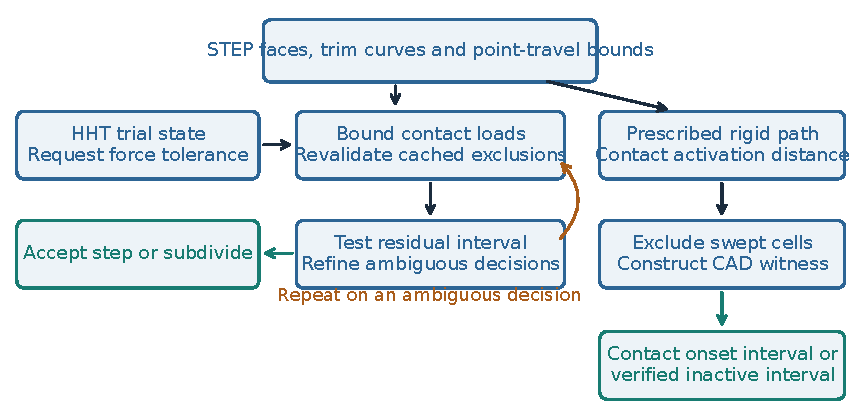
\includegraphics[width=.92\linewidth]{workflow.pdf}
\caption{Geometry queries on the original CAD boundary. The implicit solver controls the accuracy of the contact forces. The prescribed-motion query bounds contact onset.}
\label{fig:workflow}
\end{figure}

Let $Q$ denote the generalized configuration and $g_i(Q)$ the gap for contact pair or prescribed probe $i$. We use a frictionless normal force of the form
\begin{equation}
 \lambda_i(Q)=k_i [s_i-g_i(Q)]_+, \qquad
 F(Q,V,t)=F_{\mathrm{ext}}(Q,V,t)+\sum_i J_i(Q)^\top\lambda_i(Q),
 \label{eq:contact}
\end{equation}
where $s_i$ is the contact activation distance, $k_i$ is the stiffness, $J_i$ maps generalized velocities to relative normal motion, and $[b]_+=\max(0,b)$. The force activates as the pair moves into the contact layer $g_i<s_i$. Contact onset refers to the boundary of that layer. The primitive kernels use support points on spheres, cylindrical faces and finite planes. For a gear pair, the model prescribes candidate tooth pairs using the line of action. At each axial section, rays in the line-of-action direction intersect the two tooth profiles. The gap is the difference of ray coordinates multiplied by the cosine of the base helix angle. The axial quadrature and smooth shoulder weights at tooth entry and exit multiply the local stiffness. The angular lever arms follow the base radii projected by the same cosine. This model provides a normal force and an axial force component for each stage. Rigid axes carry the resulting projected torque, and the transmission stage has one shared shaft coordinate with its successor.

\subsection{Enclosing a gear section intersection}
\label{sec:gear-root}
The importer converts each sampled nonrational cubic flank section into B\'ezier spans. For a section $C(u)$, prescribed probe origin $p$, ray direction $n$ and transverse direction $w$, write $f(u)=w^\top(C(u)-p)$ and $h(u)=n^\top(C(u)-p)$. We seek the root of $f$ within the section and report $h$ there. Each B\'ezier control hull bounds the image of its span. If a global derivative bound is inconclusive, we exclude spans whose projected control hull misses the ray. We then bound $f'$ and $h'$ on the contiguous interval containing the surviving spans. Opposite signs at the ends and a one-sided $f'$ establish that the interval has a unique root $u^*$. For any $\hat u$ in the same interval the mean value theorem gives
\begin{equation}
 |h(u^*)-h(\hat u)| \leq \frac{\sup |h'|}{\inf |f'|}\, |f(\hat u)|.
 \label{eq:probe-error}
\end{equation}
We evaluate the right-hand side and the distance to the finite ray limits with outward-rounded intervals. A Newton root estimate supplies $\hat u$ when a previously evaluated point fails the current test. A span containing both the estimate and a sign change supplies tighter derivative bounds if needed. The stored point enclosure can propose a ray-coordinate interval at a new trial, where the root-existence, derivative and ray-limit checks apply again. We propagate the two accepted ray intervals through Eq.~\eqref{eq:contact}. A force-acceptable interval whose gap bound overlaps the sampled clearance floor is evaluated more tightly. The enclosures refer to the nominal extracted section polynomials. The gear model applies the local gap check at the sampled sections and trial states.

\section{Residual-controlled implicit integration}
\label{sec:method}
We use HHT-$\alpha$ for the reduced rigid coordinates, with $\alpha=-0.10$ in the reported runs. With a step size $\Delta t$, constant generalized mass $M$, and $a$ as the next acceleration, the predictors give $Q_{n+1}=Q_p+\beta\Delta t^2 a$ and $V_{n+1}=V_p+\gamma\Delta t a$, where $\beta=(1-\alpha)^2/4$ and $\gamma=1/2-\alpha$. The discrete force residual is
\begin{equation}
 R(a)=Ma-(1+\alpha)F(Q_{n+1},V_{n+1},t_{n+1})+\alpha F_n .
 \label{eq:residual}
\end{equation}
The force oracle accepts an absolute error budget $\eta_{\mathrm{req}}$ and returns $\widehat F$ and a bound $\eta$ on $\norminf{F-\widehat F}$. The accepted previous state retains its force bound $\eta_n$. The computed residual therefore differs from the nominal residual by at most
\begin{equation}
 \norminf{R-\widehat R} \leq |1+\alpha|\eta+|\alpha|\eta_n.
 \label{eq:resid-error}
\end{equation}
The implementation additionally encloses arithmetic in Eq.~\eqref{eq:residual} and bounds the norm componentwise in the numerical scaling of the generalized coordinates. If $[r^-,r^+]$ is the resulting interval for $\norminf R$, the trial converges whenever $r^+$ is at most the lower bound of the prescribed absolute-plus-relative tolerance. A trial with $r^-$ above the upper tolerance bound needs another Newton iteration. An overlap requests a tighter force estimate, as in Fig.~\ref{fig:residual}. A line search certifies descent only if the next residual upper bound is below the current lower bound. It refines the next interval, then the current interval if necessary, before re-evaluating that test. Algorithm~\ref{alg:trial} summarizes the solver.

\begin{figure}[pos=!htbp]
\centering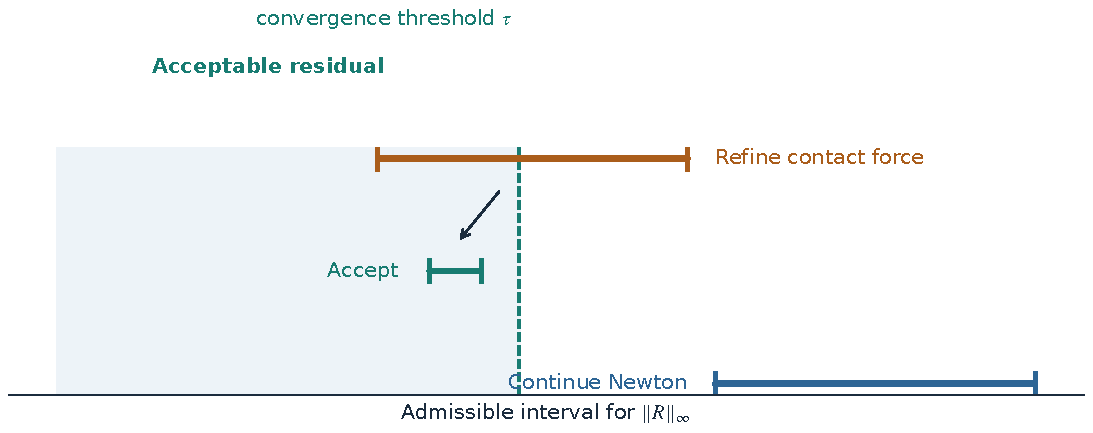
\includegraphics[width=.89\linewidth]{principle-residual.pdf}
\caption{Contact-force accuracy is sufficient when the residual interval decides the Newton test. An interval that overlaps the convergence threshold triggers a tighter force evaluation. During a line search the criterion tests the ordering of two residual intervals.}
\label{fig:residual}
\end{figure}

The first force budget scales with the prior force. Later budgets scale with the current residual, using the fraction $0.1$ after mapping through $1+\alpha$. Tight evaluation uses the finest available oracle. For primitive contact pairs, a lower gap bound $L_i>0$ and a bound $S_i$ on the normal Jacobian give the force contribution bound $k_i[s_i-L_i]_+S_i$. We sort unresolved contributions by this bound and may omit a tail when the sum of its bounds lies within the requested force budget. The actual force error includes the omitted sum and the interval widths of the evaluated contributions. The solver uses this actual error when the oracle exceeds the requested target. If the available precision cannot resolve an acceptance decision, the step may be subdivided within the prescribed limit.

\begin{algorithm}[!htbp]
\caption{HHT trial step with bounded contact evaluation}
\label{alg:trial}
\begin{algorithmic}[1]
\Require Prior state and force enclosure, time step $\Delta t$, residual tolerances
\State Form HHT predictors and set the trial acceleration from the prior state
\For{each allowed Newton iteration}
  \State Revalidate inactive-pair bounds at the trial configuration
  \State Evaluate contact loads using the requested budget and bound $\norminf R$
  \If{the residual interval overlaps the convergence tolerance}
     \State Request the finest available force evaluation and update the interval
  \EndIf
  \If{the upper residual bound satisfies the lower tolerance bound}
     \State \Return trial state and force bound if the applicable gap test also passes
  \EndIf
  \State Form the Newton direction from the current force tangent
  \State Check line-search trials and tighten overlapping residual intervals as needed
  \State Use the first trial with certified descent, or leave the iteration on failure
\EndFor
\State Subdivide the step if the subdivision budget remains
\end{algorithmic}
\end{algorithm}

\subsection{Reusing an exclusion}
A lower bound $L_0$ for the gap at configuration $Q_0$ remains useful at a nearby trial $Q$. For each body, let $d_A$ or $d_B$ bound the travel of every one of its material points between the two configurations. A translation contributes its magnitude and a rotation through $\Delta\theta$ about a fixed axis contributes at most $r |\Delta\theta|$, where $r$ bounds the distance of the surface from that axis. The triangle inequality holds for every point pair, so taking the infimum yields
\begin{equation}
 d(A(Q),B(Q)) \geq L_0-d_A-d_B.
 \label{eq:transport}
\end{equation}
If this lower bound exceeds $s_i$, the pair is inactive at $Q$. The cache stores its configuration and original lower bound. A trial outside the validity region in Fig.~\ref{fig:reuse} calls the ordinary gap query. A rejected trial cannot create a false exclusion because any stored state is rechecked according to Eq.~\eqref{eq:transport}. For linearly interpolated reduced coordinates on supported primitive pairs, each intermediate point is within half of the total step travel of one endpoint. The smaller endpoint lower bound minus half the total relative travel is therefore a conservative lower bound for the segment.

\begin{figure}[pos=!htbp]
\centering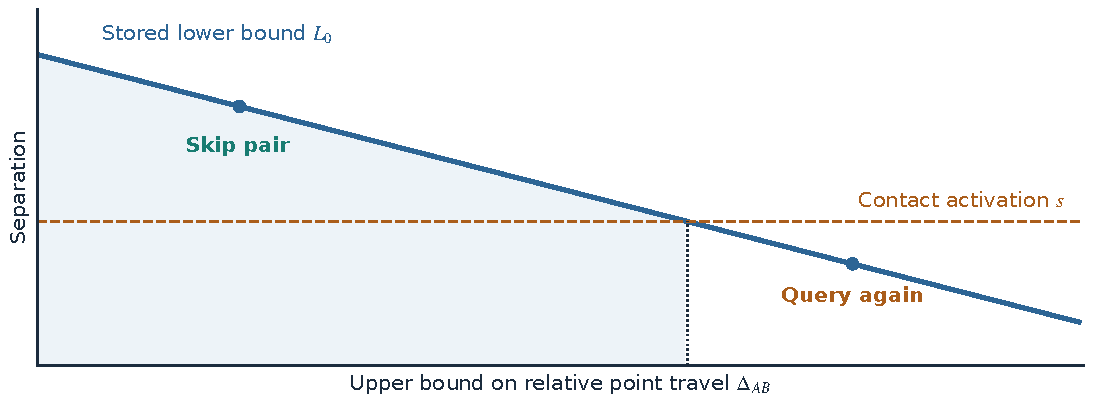
\includegraphics[width=.89\linewidth]{principle-reuse.pdf}
\caption{Validity of a stored separation bound at later Newton trials. The displacement bound can invalidate an exclusion as relative point travel grows.}
\label{fig:reuse}
\end{figure}

\section{Contact onset on a prescribed motion}
Consider a stationary boundary $A$ and a moving boundary $B(t)$ under a fixed-axis rotation with an affine translation. For a pair that starts outside the contact layer, the onset time is $t^*=\inf\{t:d(A,B(t))\leq s\}$, with $s$ the contact activation distance. The search combines enclosures of trimmed CAD cells with directional bounds on their relative motion. It excludes cells whose distance lower bound exceeds $s$ and processes the remaining cell-time windows in increasing order of start time. When the bounds are inconclusive the search splits cells or the time interval. A globally verified inactive interval ends at $t_-$. At any time $t_+$, a feasible CAD point pair whose outward distance upper bound is at most $s$ establishes $t^*\leq t_+$. The verification uses the point positions on the CAD, regardless of how they were proposed.

The interval search can advance the lower bound even when sampled points miss the region where contact begins. When a pair of trimmed cells survives the lower-bound tests, the general search evaluates feasible point pairs at the endpoints and midpoint of the surviving time window. The routine verifies both point parameters on the original boundary and tests their distance before updating $t_+$. At the work limit the search reports the verified inactive interval and any available upper time bound. Figure~\ref{fig:event-schematic} illustrates these results.

\begin{figure}[pos=!htbp]
\centering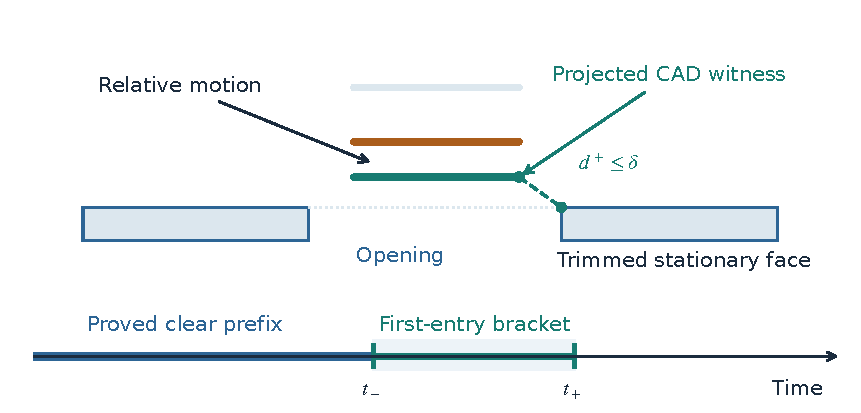
\includegraphics[width=.89\linewidth]{principle-event.pdf}
\caption{Bounding contact onset near a planar trim. A verified inactive interval ends at $t_-$, and the CAD point pair at $t_+$ satisfies the contact criterion.}
\label{fig:event-schematic}
\end{figure}

\subsection{Software interfaces}
The C++20 implementation separates geometry preparation, prescribed-motion search, and force evaluation. Prepared geometry is reused as poses and trajectory parameters change. The prescribed-motion query exposes the end of the verified inactive interval, an optional point pair with enclosing positions, and work counters. The force callback supplies force, stiffness, damping, and error information in the integrator's generalized coordinates. It also supports direct force evaluation for comparison. The verification tests check accepted residuals against a separate force evaluation, oracle behavior under a limit on attainable precision, and STEP import and query behavior.
